\documentclass{article}
\usepackage{amsmath, amssymb, mathrsfs, kotex, hyperref, graphicx, mdframed, setspace,enumitem}
\usepackage[a4paper, margin = 40pt]{geometry}
\setstretch{1.5}
\newcommand\ar{\ensuremath{\text{AR}}}
\newcommand\ma{\ensuremath{\text{MA}}}
\newcommand\arma{\ensuremath{\text{ARMA}}}
\newcommand\cov{\ensuremath{\text{Cov}}}
\newcommand\sa{\ensuremath{{\sigma_a}^2}}

\begin{document}
\title{Arima Model - 6}
\author{강의 : 김성범 교수님\\ 정리 :  김선중}
\date{\today}
\maketitle

이것은 \href{https://youtu.be/K7GWJ3iC6OY}{ARIMA 모델 개요 - Part 6} 강의에 대한 노트이다.
이번 내용은 계산이 많으므로, 설명을 길게 쓰는 것보다는 계산을 나열하는 것 위주로 정리했다.
다만, conditional expectation과 prediction interval에 대해서는 조금 공부해야 할 것 같아서 앞에 적어보있다.
지난 번에는 영어로 적었었는데, 이번에는 다시 한글로 적었다.
\tableofcontents

\newpage
\begin{center}
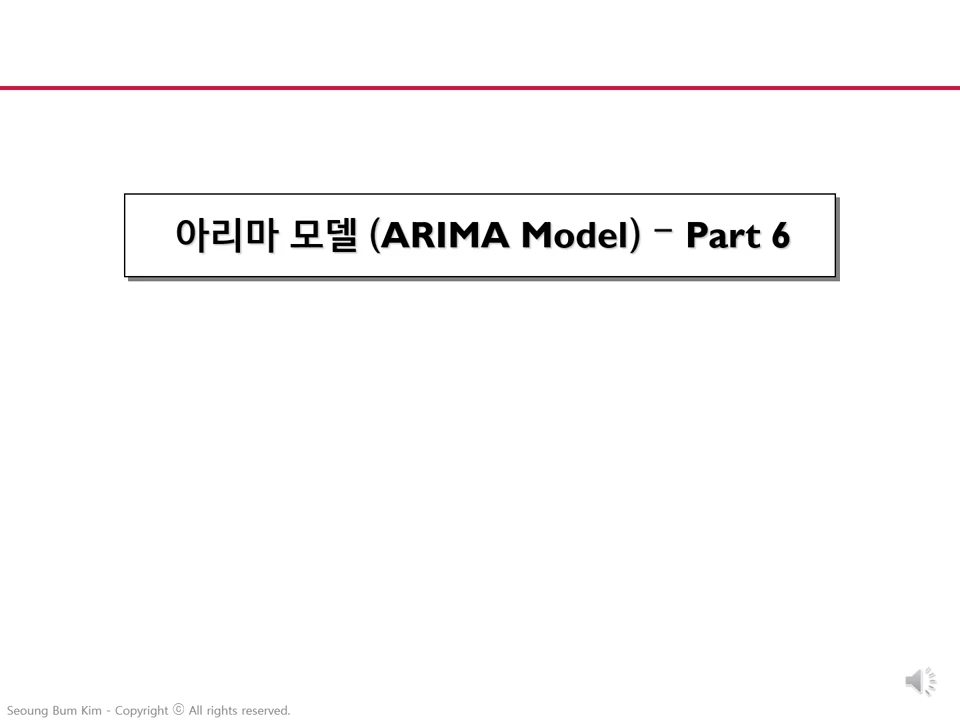
\includegraphics[width=.45\textwidth]{capture_01}
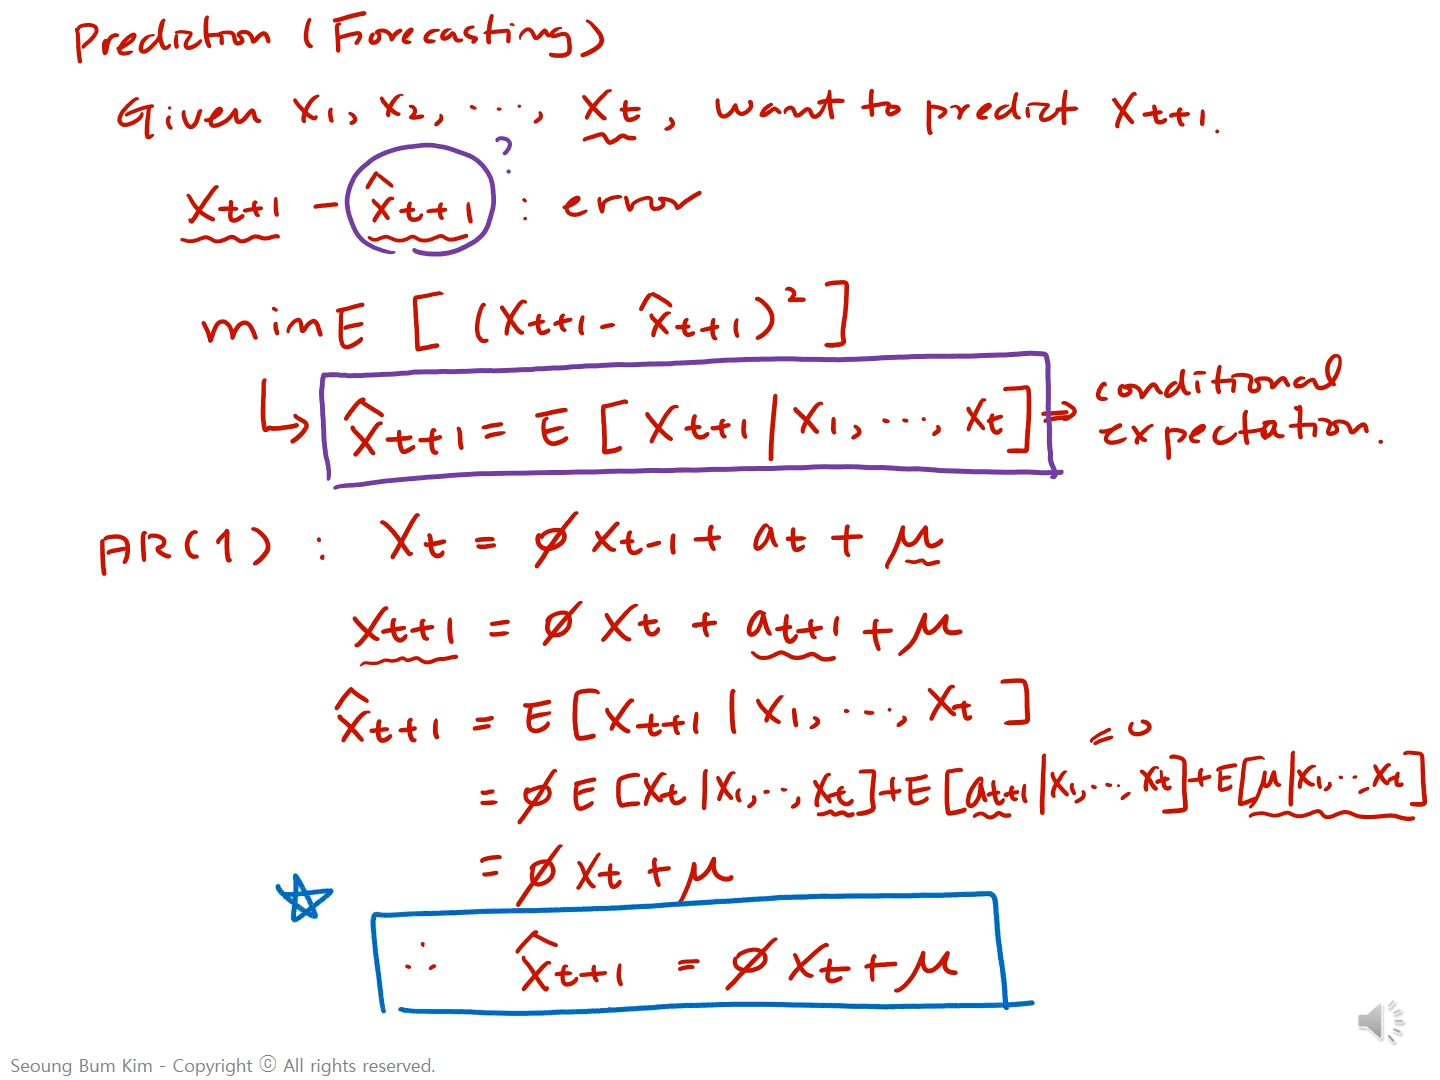
\includegraphics[width=.45\textwidth]{capture_02}
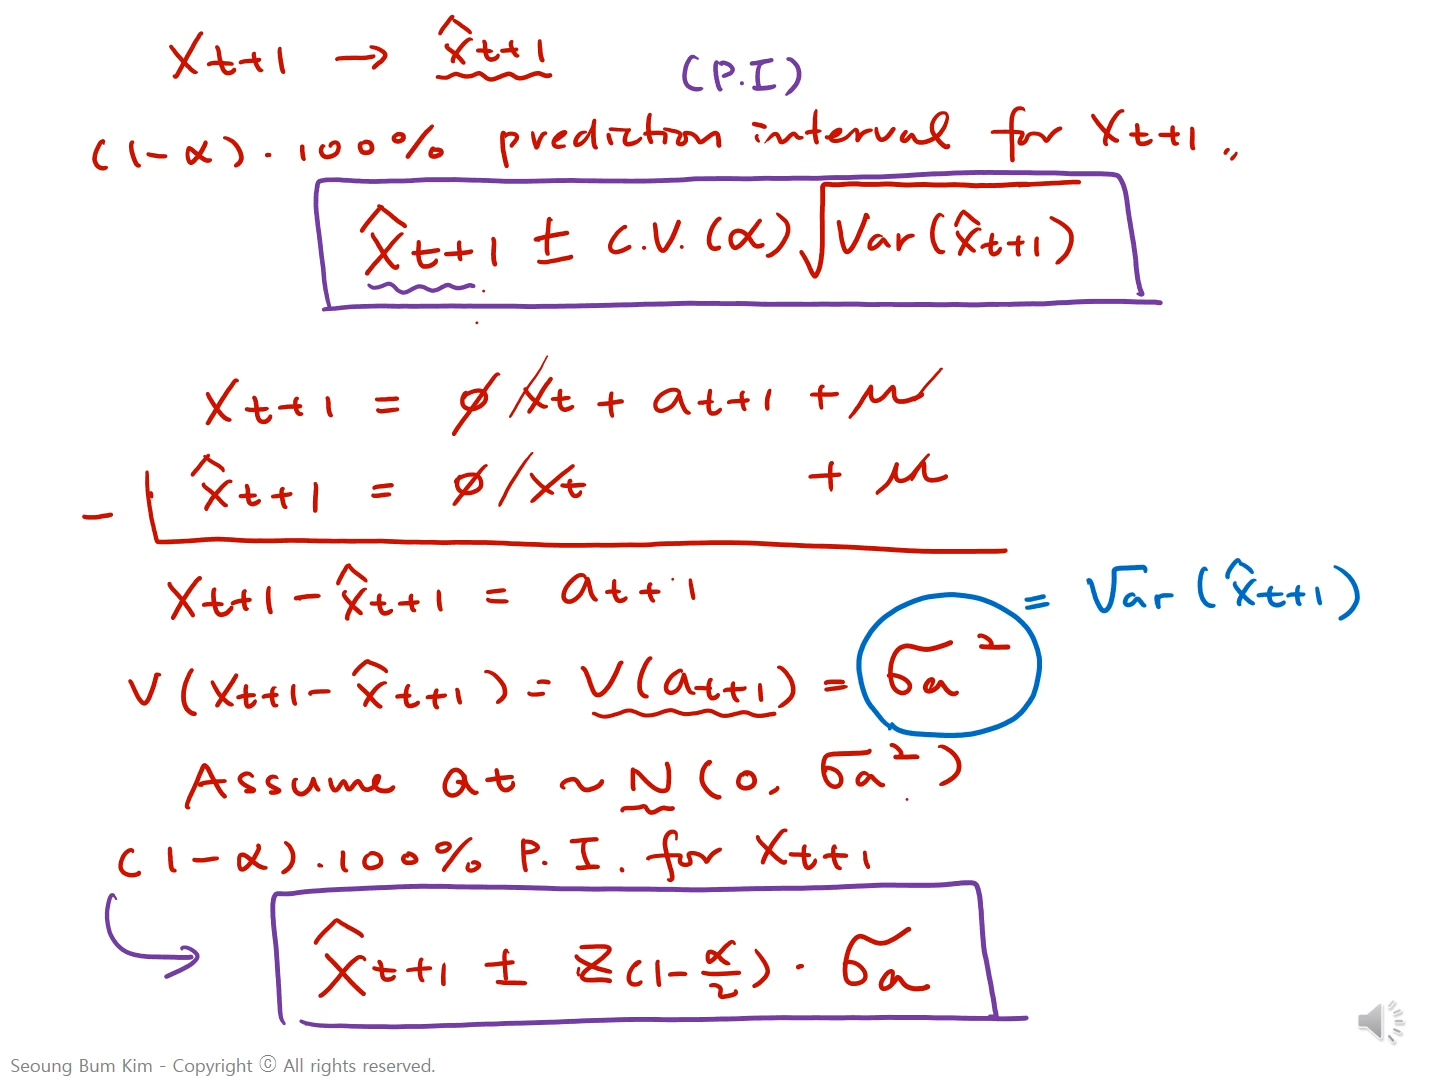
\includegraphics[width=.45\textwidth]{capture_03}
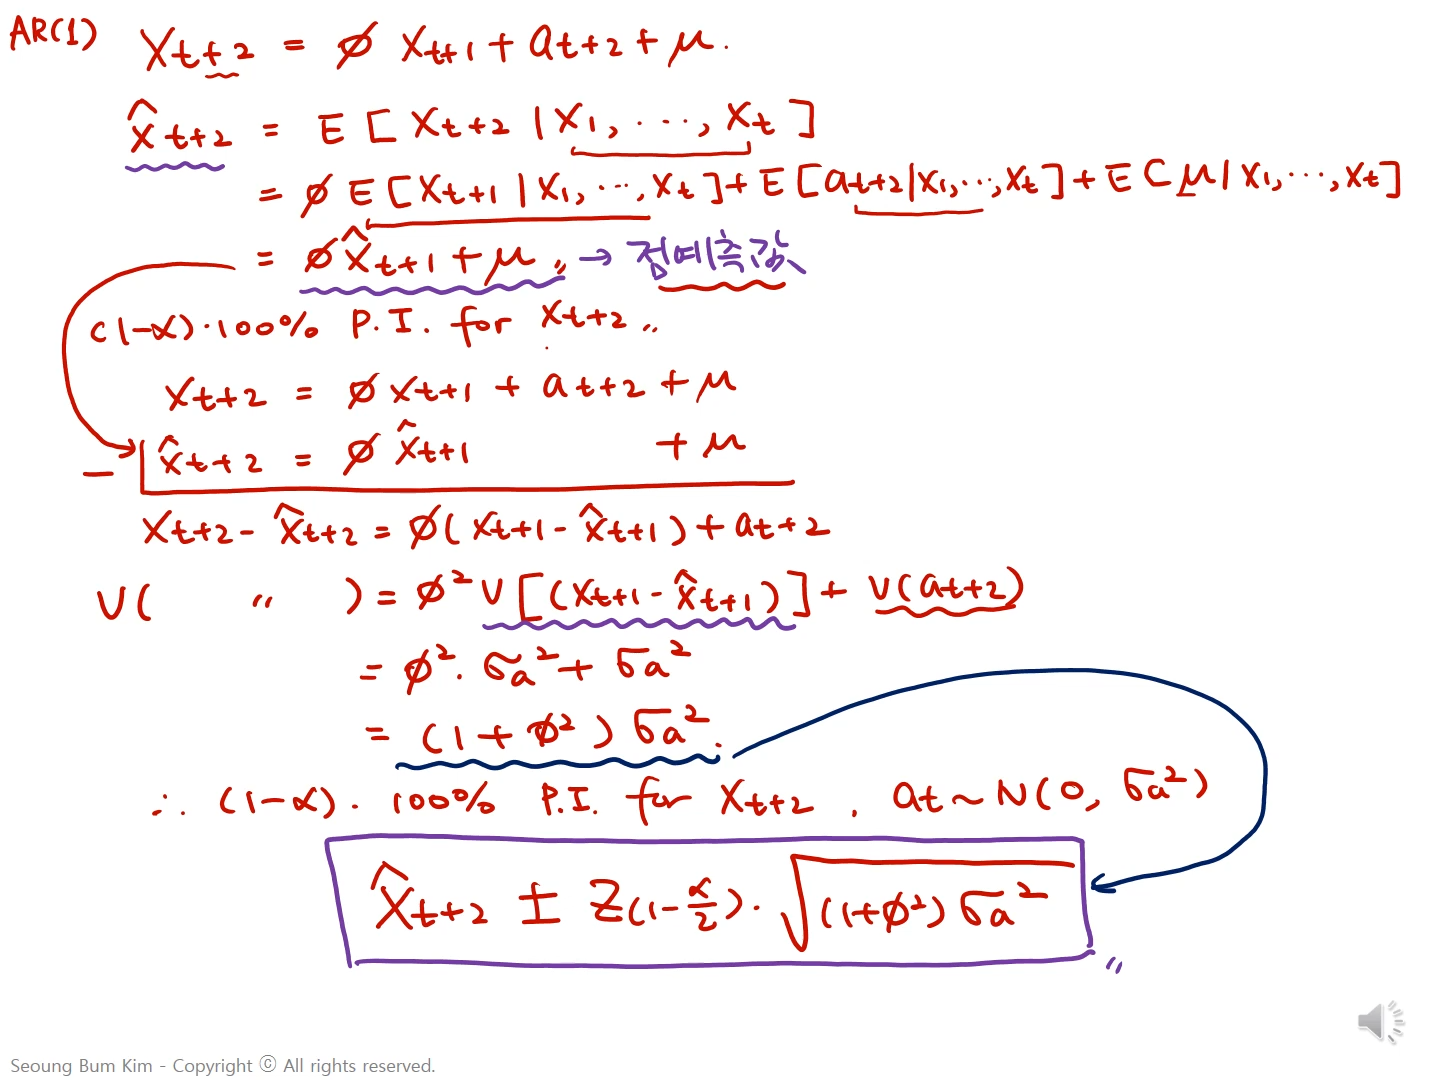
\includegraphics[width=.45\textwidth]{capture_04}
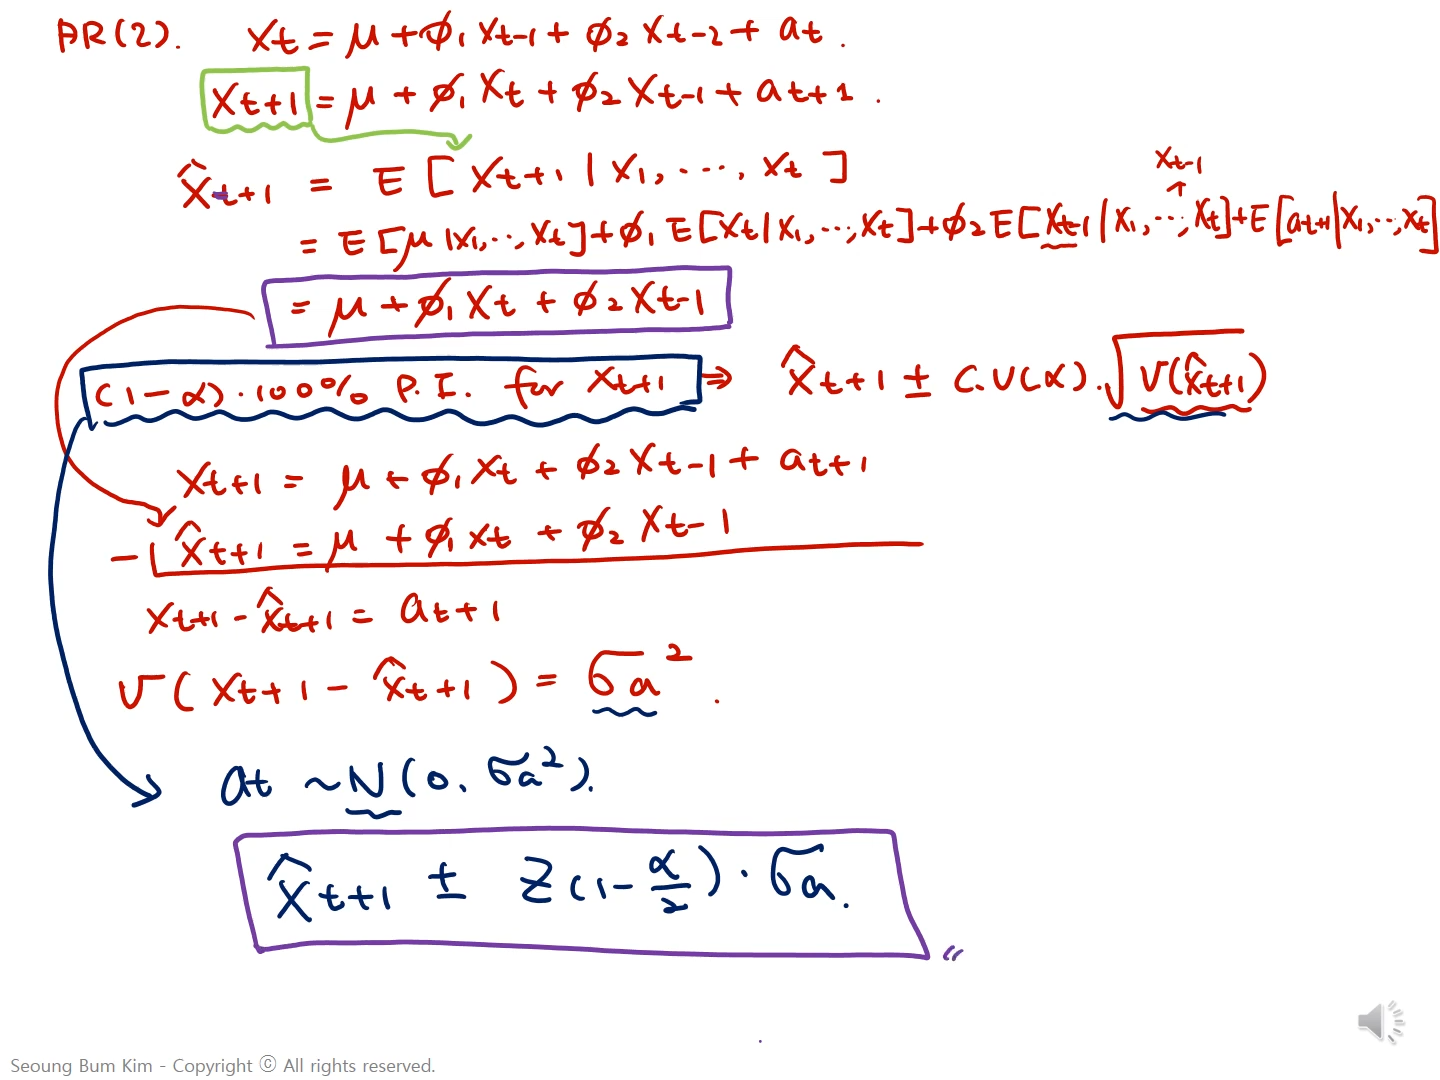
\includegraphics[width=.45\textwidth]{capture_05}
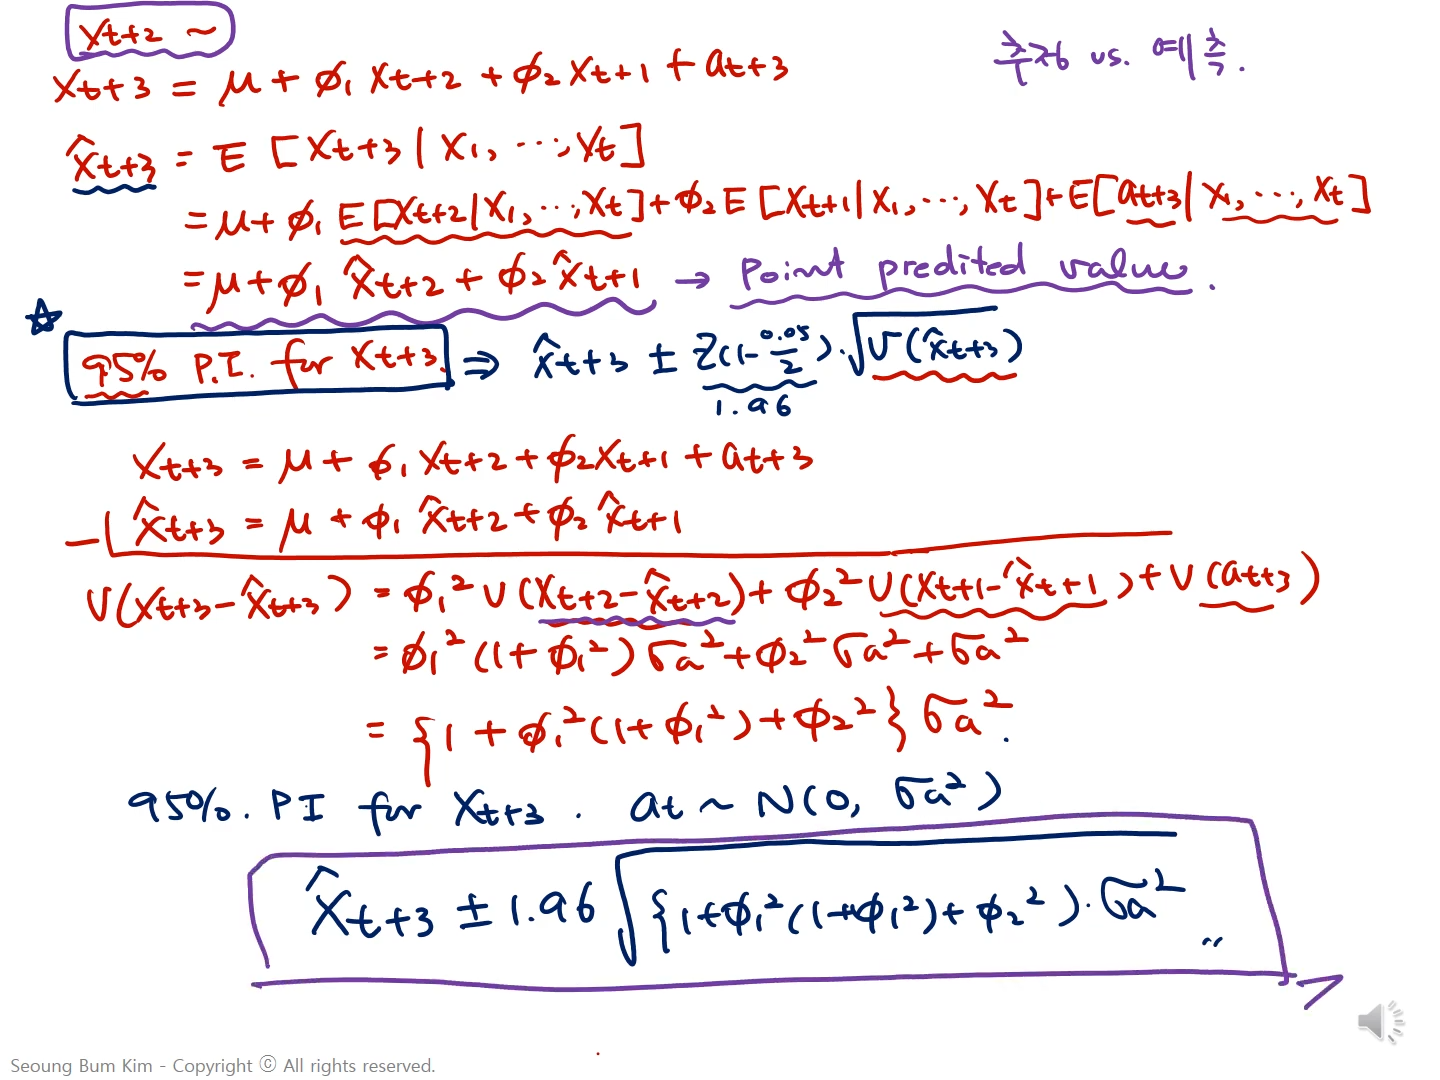
\includegraphics[width=.45\textwidth]{capture_06}
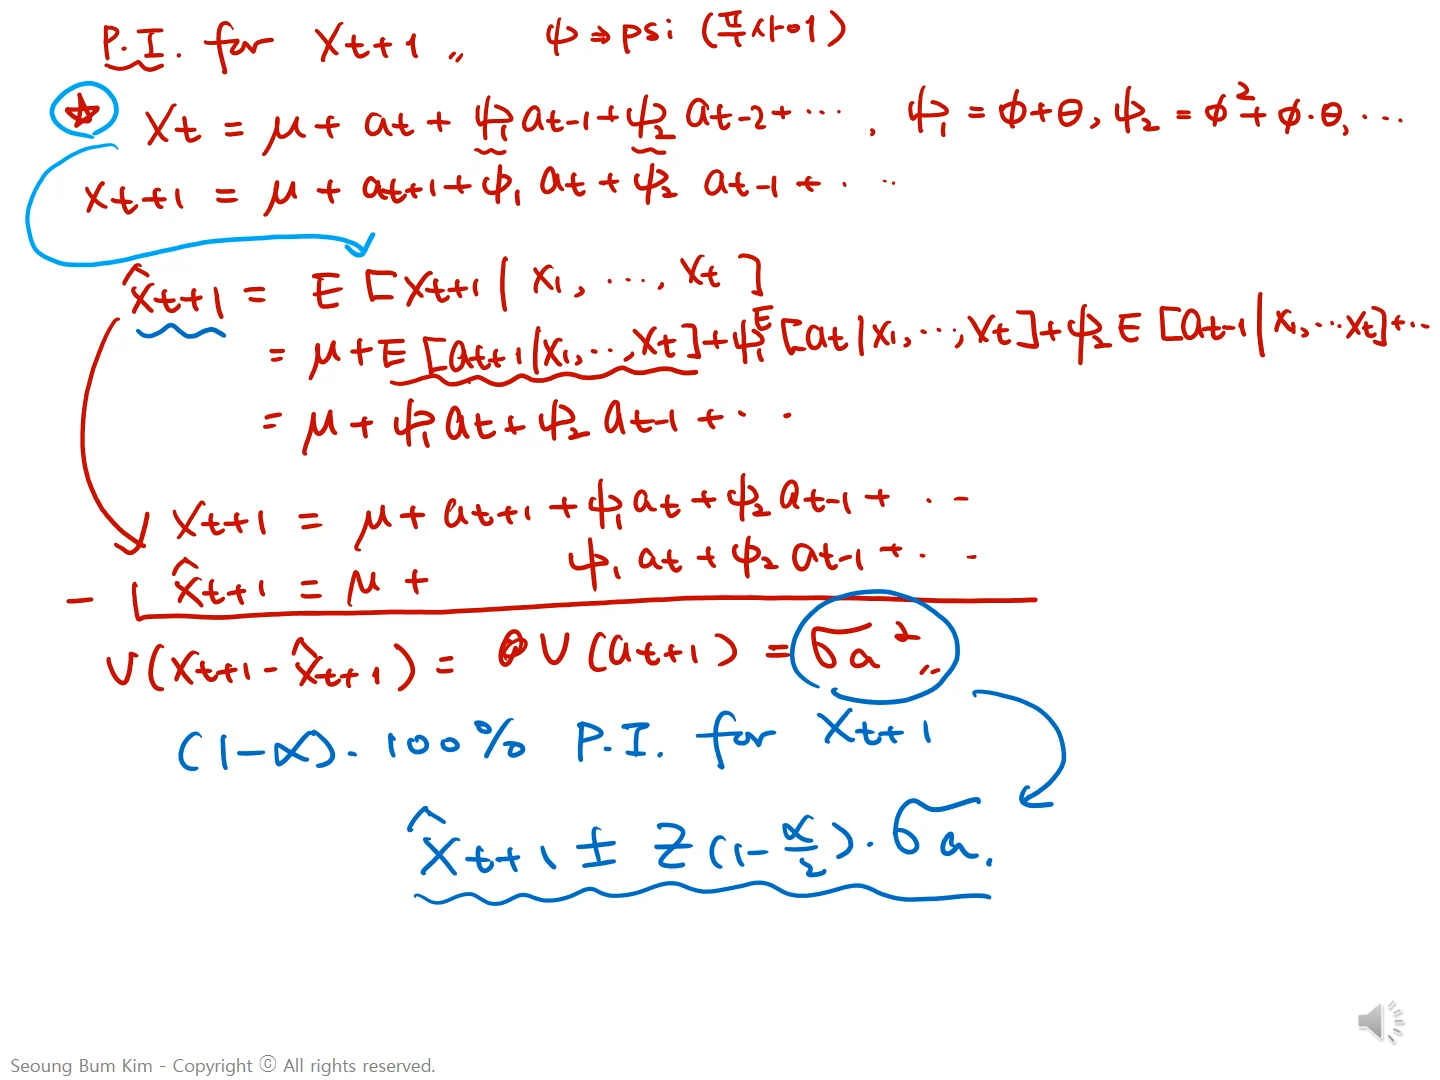
\includegraphics[width=.45\textwidth]{capture_07}
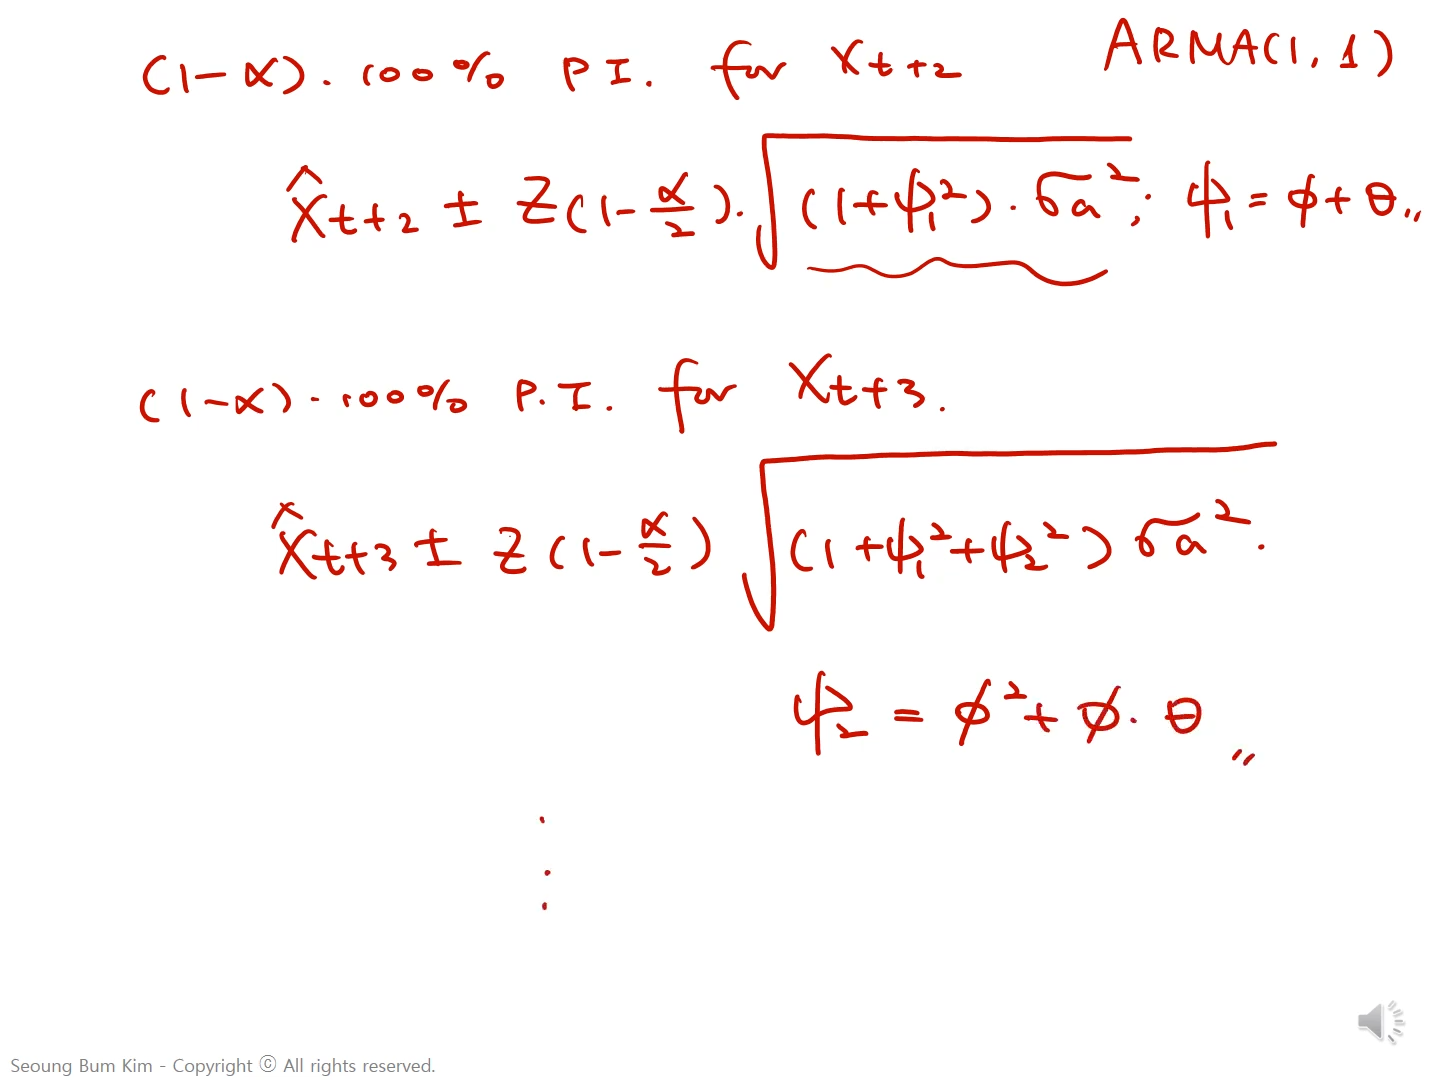
\includegraphics[width=.45\textwidth]{capture_08}
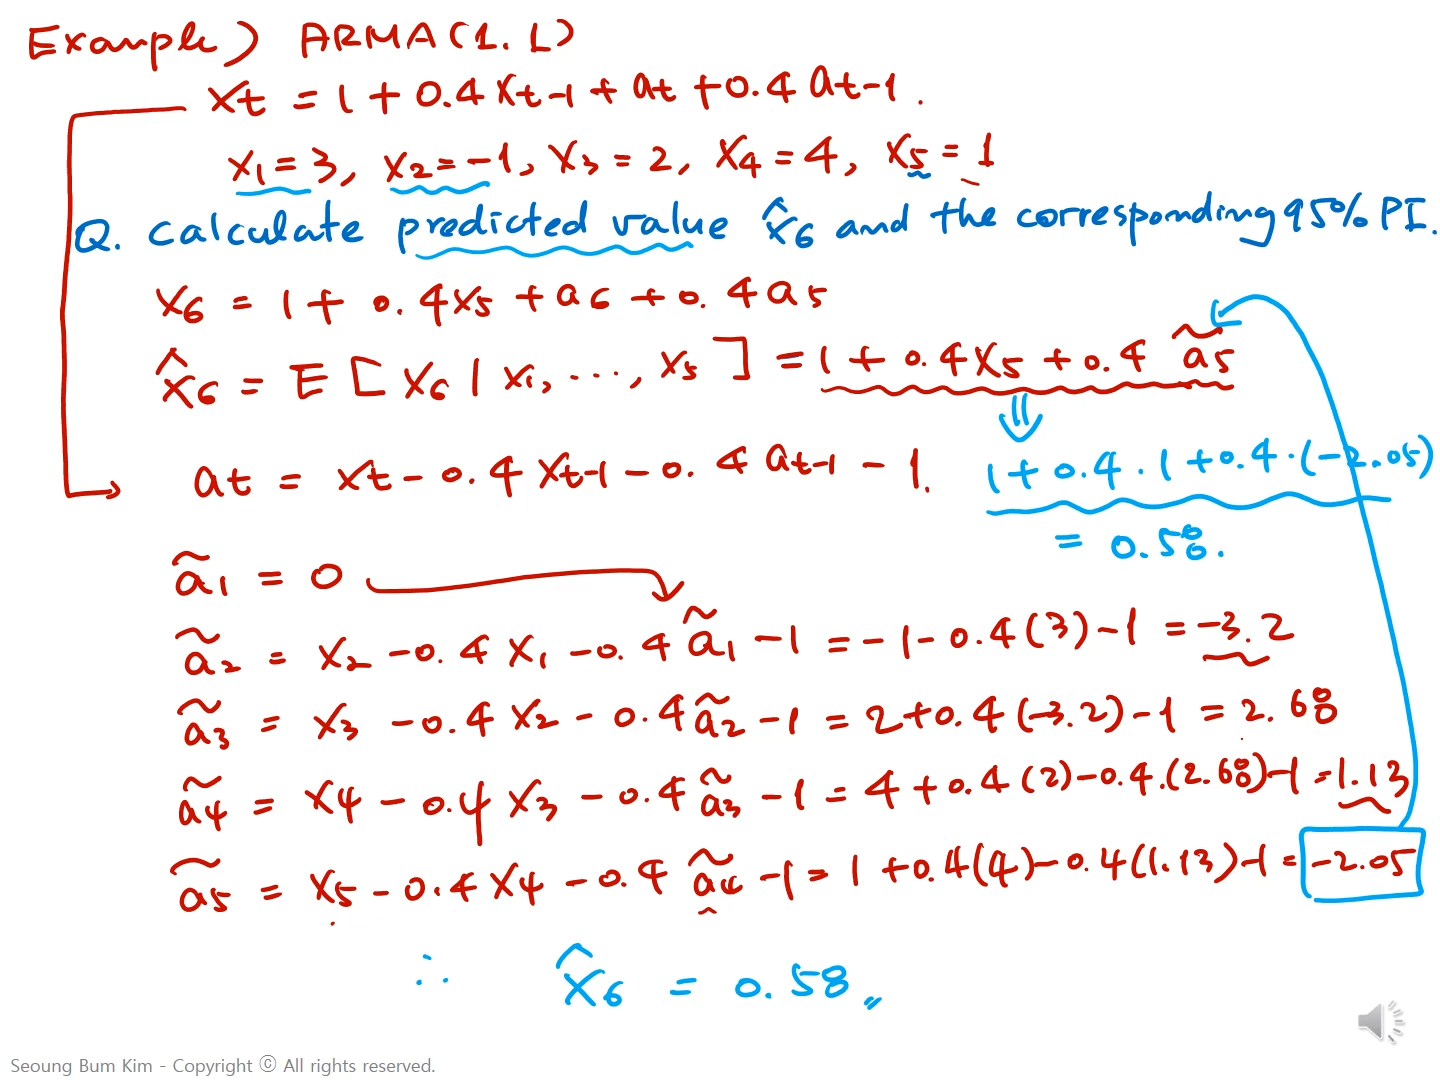
\includegraphics[width=.45\textwidth]{capture_09}
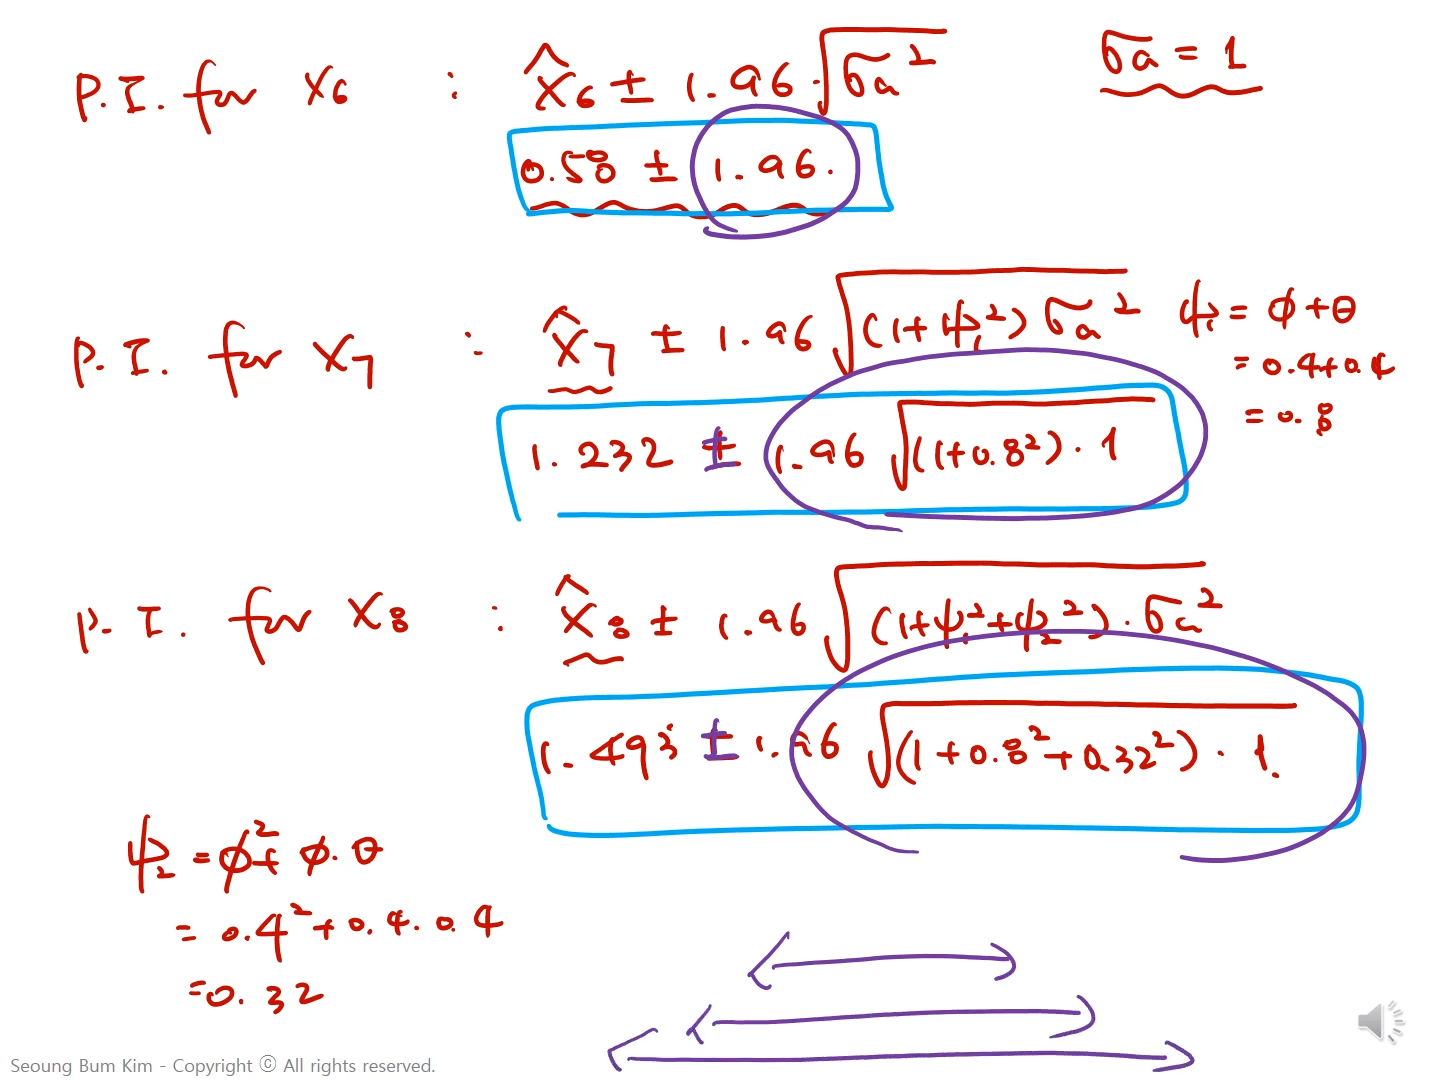
\includegraphics[width=.45\textwidth]{capture_10}
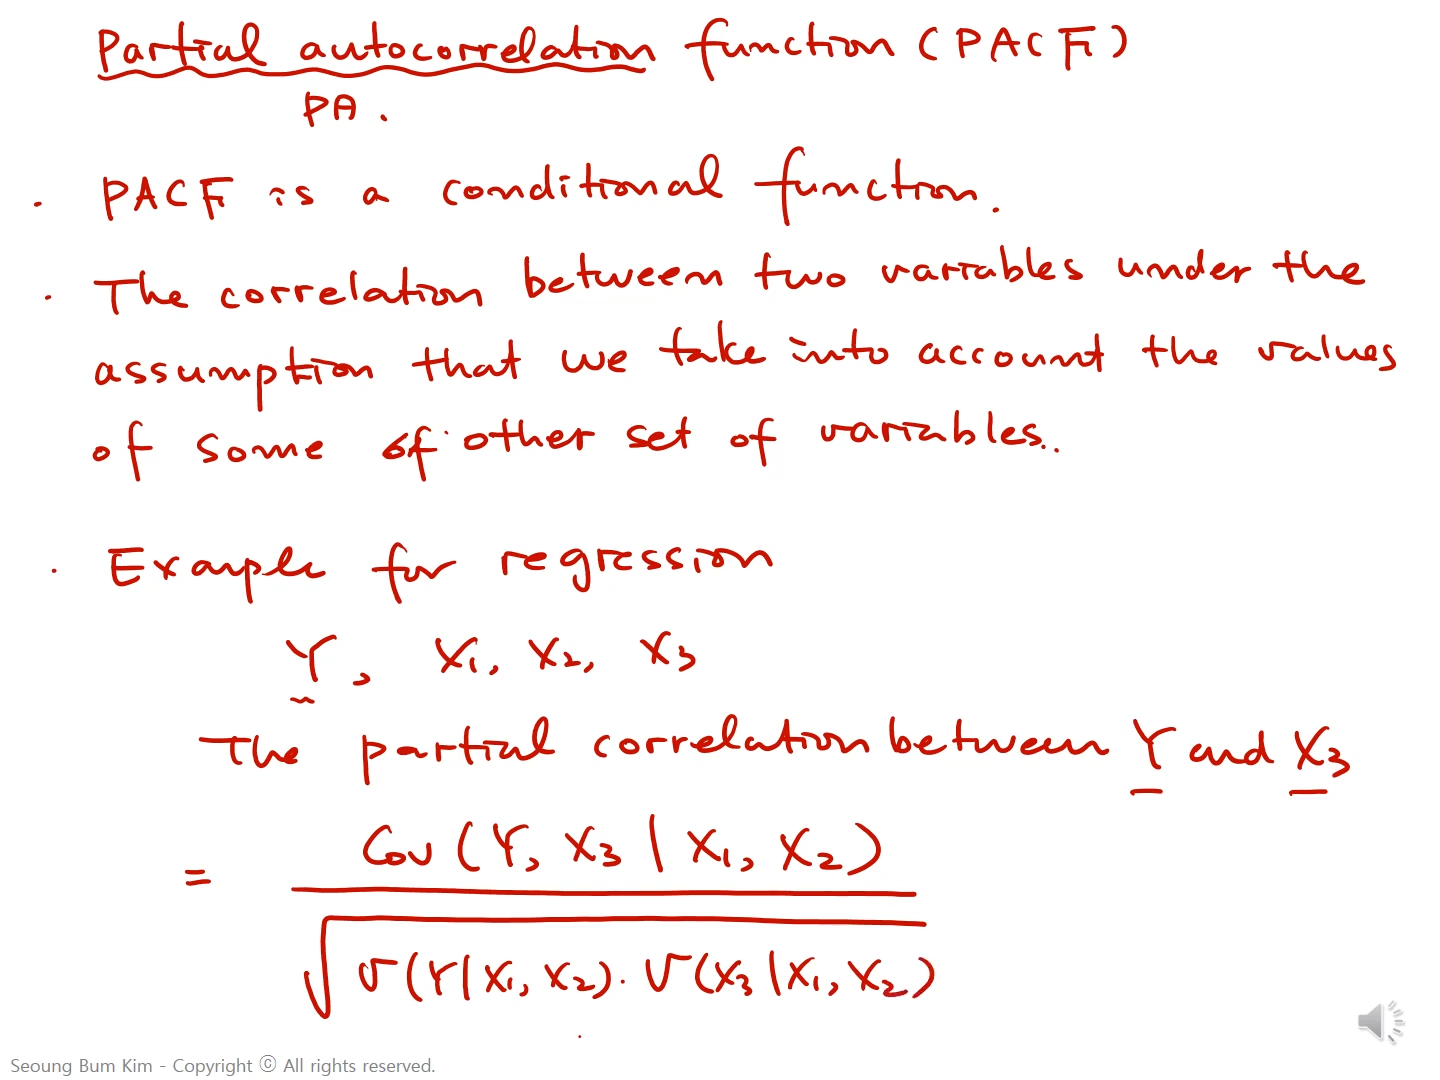
\includegraphics[width=.45\textwidth]{capture_11}
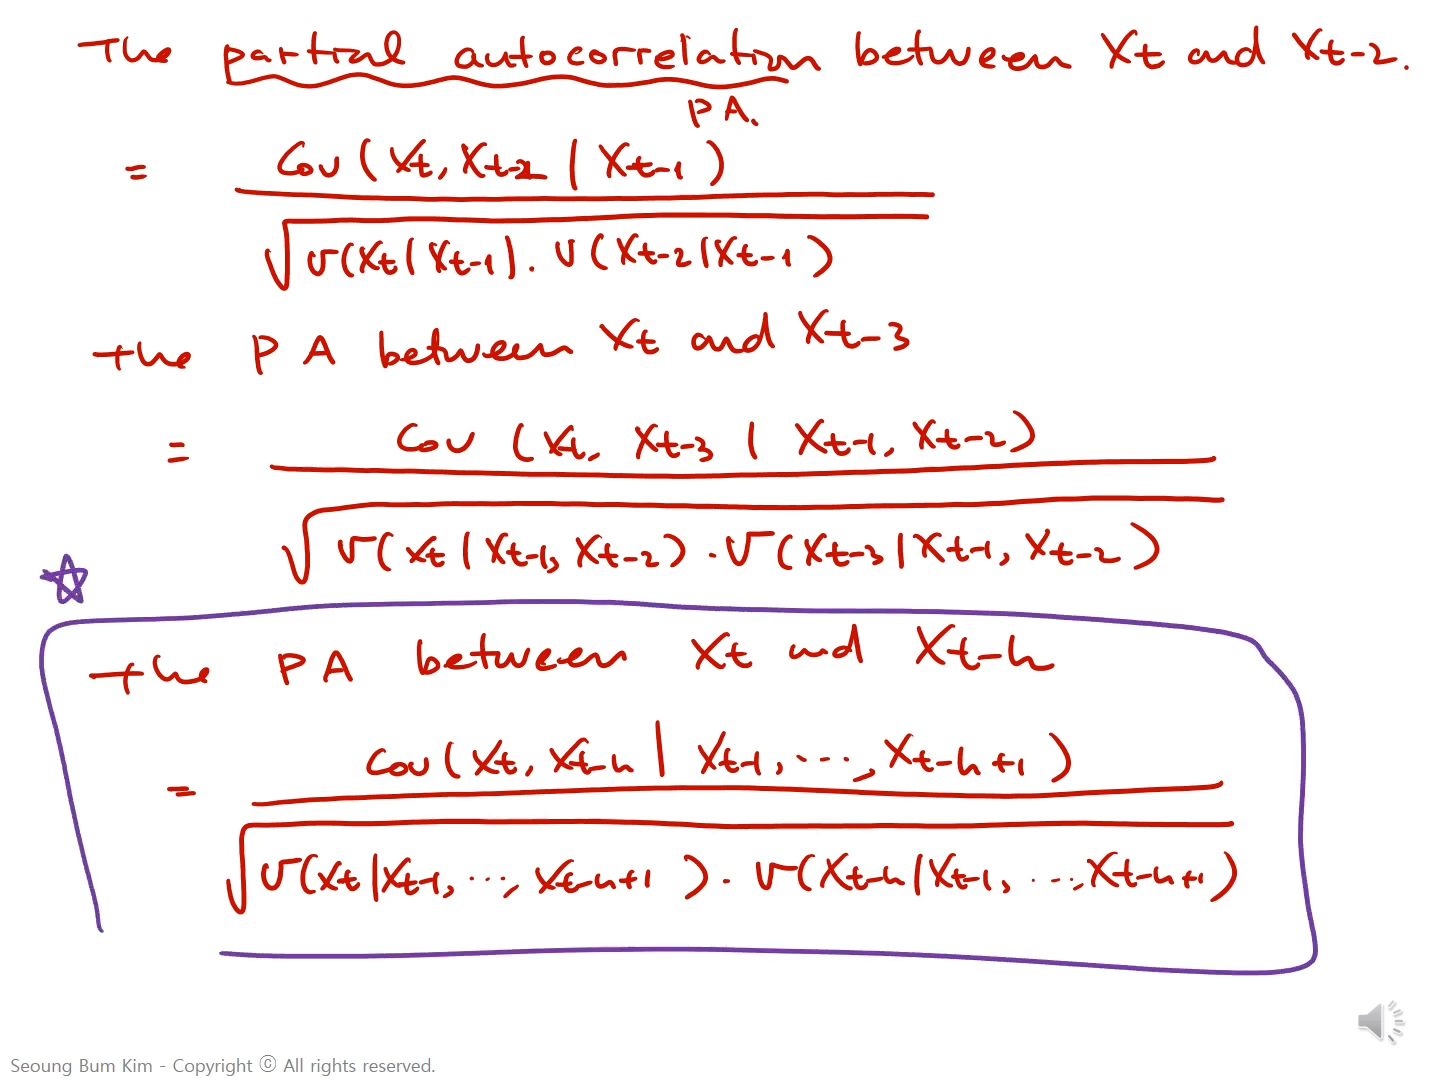
\includegraphics[width=.45\textwidth]{capture_12}
\end{center}

%%%
\section{Preliminaries}

%%
\subsection{Conditional Expectations}

Conditional expectation에 관해서는 \href{https://www.math.arizona.edu/~tgk/464_07/cond_exp.pdf}{이 자료(A Conditional expectation - Arizona Math)}참조했다.
해당 자료의 A.1, A.2를 옮겨서 적으려고 했다.
그런데, 적다보니 확률론에 관한 일반적인 사실을 많이 적게 되었다.
사실 하고 싶었던 건 conditional expectation에 대해 정확하게 이해하는 거였고, 또 강의내용을 잘 이해하는 거였는데, 그러자면 확률과정(stochastic process)에 대해 이해할 수 있어야 했다.
확률과정에 대해서 배운 적은 없긴 하지만, 아마 이와 비슷한 걸 알고 있으면 되는 게 아닐까 하는 생각이 있다.

그렇다고 확률론의 모든 내용을 적은 건 당연히 아니다.
예를 들어 두 사건의 독립/종속에 대해서는 안적었고 전체확률의 법칙(the law of total probability)같은 것도 안 적었다.
아무튼, 적다보니, 확률론에 대해 너무 많은 걸 적게 되었다.
그래도 이번 기회에 헷갈려했던 것들을 깔끔하게 정리하게 된 것 같다는 느낌이 든다.

%
\subsubsection{Probability Spaces and Random Variables}
확률공간 \((\Omega,\mathcal F,\mathbb P)\)을 고려하자.
늘 그렇듯이 \(\Omega\)는 표본공간(sample space)이고, \(\mathcal F\)는 사건공간(event space)이고, \(\mathbb P\)는 확률측도(probability measure)이다.
사건(event)이란, 표본 공간 \(\Omega\)의 부분집합이고, \(\mathcal F\)는 사건들의 집합이지만 모든 사건들의 집합일 필요는 없다. 그보다는, \(\mathcal F\)는 \(\Omega\)에 대한 \(\sigma\)-algebra이라서 세 가지 정도의 성질을 만족시키는 집합이다.
\(\mathbb P\)는 유한측도(finite measure)로서, \(\mathbb P:\mathcal F\to[0,1]\)인 함수이고 역시 몇가지 성질을 만족시킨다.

확률변수란 \(\Omega\)에서 \(\mathbb R\)로 가는 함수이다.
즉, \(X\)가 확률변수이면 \(X:\Omega\to\mathbb R\)이다.
이때 \(X\)의 공역이 꼭 \(\mathbb R\)일 필요는 없지만, 많은 경우에는 그렇게 하므로, 그냥 공역을 \(\mathbb R\)이라고 하겠다.

확률변수에는 이산확률변수(discrete random variable)과 연속확률변수(continuous random variable)이 있다.
확률변수 \(X\)의 치역이 이산적(discrete)이면 이산확률변수라고 하고 연속적(continuous)이면 연속확률변수라고 한다.

각각의 확률변수들은 확률분포(random distribution)을 가지고 있다.
이산확률변수의 확률분포는 이산확률분포(discrete random variable)라고 부르고, 이때의 확률분포는 확률질량함수 \(x\mapsto\mathbb P(X=x)\)로서 표현된다.
이때 확률질량함수는
\begin{itemize}
\item
\(0\le\mathbb P(X=x)\le1\)
\item
\(\sum_x\mathbb P(X=x)=1\)
\end{itemize}
을 만족하는 함수여야 한다.
연속확률변수의 확률분포는 연속확률분포(continuous random variable)라고 부르고, 이때의 확률분포는 확률밀도함수 \(f(x)\)로서 표현된다.
이때 확률밀도함수는
\begin{itemize}
\item
\(f(x)\ge0\)
\item
\(\int_xf(x)\,dx=1\)
\item
\(\int_a^bf(x)\,dx=\mathbb P(a\le X\le b)\)
\end{itemize}
를 만족하는 함수여야 한다.

예를 들어, 주사위를 하나 던지는 시행을 생각하자.
그러면 표본공간은 \(\Omega=\{1,2,3,4,5,6\}\)이고, 사건공간은 \(\mathcal F\)는 \(\Omega\)의 멱집합, 즉 \(\Omega\)의 모든 부분집합들의 집합으로 둘 수 있다.
즉,
\[\mathcal F=2^\Omega=\left\{\varnothing,\{1\},\{2\},\cdots,\{1,2,3,4,5,6\}\right\}\]
이다.
그리고, 확률측도 \(\mathbb P\)는, \(A\in\mathcal F\)에 대하여
\[\mathbb P(A)=\frac{|A|}{|\Omega|}\]
이다.
다시 말해서, \(A=\{1,2\}\)이면
\[\mathbb P(A)=\frac{|\{1,2\}|}{|\{1,2,3,4,5,6\}|}=\frac26=\frac13\]
이 된다.
주사위를 하나 던졌을 때 나온 눈을 2로 나누었을 때의 나머지를 \(X\)라고 하면, 이 확률변수는 하나의 함수 \(X:\{1,2,3,4,5,6\}\to\mathbb R\)로서
\[\begin{cases}
X(1)=1\\
X(2)=0\\
X(3)=1\\
X(4)=0\\
X(5)=1\\
X(6)=0\\
\end{cases}\]
로 정의된다.
\(X\)의 역은 \(\{0,1\}\)이므로 \(X\)는 이산확률변수이고, 확률질량함수는
\[\begin{cases}
\mathbb P(X=0)=\frac12\\
\mathbb P(X=1)=\frac12
\end{cases}\]
가 된다.

두번째 예로서, 수직선 위의 구간 \([0,6]\)에서 임의로 하나의 숫자를 선택하는 시행을 고려하자.
그러면 표본공간은 \(\Omega=[0,6]\)이다.
사건공간 \(\mathcal F\)에 대해 설명하는 건 좀 복잡하다.
아까처럼 \(\mathcal F\)가 \(\Omega\)의 모든 부분집합들의 집합일 수는 없다.
\footnote{아마 그러면 안될 것이다. 이유가 뭐였더라, 아마도 cantor set 같은게 문제가 됐던 것 같은데.}
\(\mathcal F\)는 \(\Omega\)의 보렐집합(borel set)이어야 한다.
다시 말해서 \(\Omega=[0,6]\)의 standard topology를 \(\mathcal T\)라고 할 때,
\[\mathcal F=\bigcap\{\mathcal S\supset\mathcal T:\mathcal S\text{ is a \(\sigma\)-algebra of \(\Omega\)}\}\]
이다.
확률측도 \(\mathbb P\)는 아까와 비슷하게 정의된다.
\(A\in\mathcal F\)에 대하여
\[\mathbb P(A)=\frac{|A|}{|\Omega|}\]
다만 아까 \(|A|\)가  집합 \(A\)의 원소의 개수(cardinality)를 의미했다면, 이번의 \(|A|\)는 집합 \(A\)의 길이, 즉, \(\mathbb R\)의 Lebesgue measure이다.
다시 말해서 \(A=[0,2]\in\mathcal F\)에 대하여
\[\mathbb P(A)=\frac{|[0,2]|}{|[0,6]|}=\frac26=\frac13\]
이다.
\([0,6]\)에서 임의로 하나 고른 숫자를 2로 나눈 값을 \(X\)라고 하면, 이 확률변수는 하나의 함수 \(X:[0,6]\to\mathbb R\)로서
\[X(t)=\frac t2\quad(0\le t\le6)\]
로 정의된다.
\(X\)의 치역은 \([0,3]\)이므로 \(X\)는 연속확률변수이고, 확률질량함수는
\[f(x)=\frac13\quad(0\le x\le3)\]
이 된다.

%
\subsubsection{Expectations}
이산확률변수 \(X\)에 대하여 기댓값(expectation) \(\mathbb E[X]\)은
\[\mathbb E[X]=\sum_xx\mathbb P(X=x)\]
이다.
%이때, \(x\mapsto\mathbb P(X=x)\)는 확률질량함수(probability mass function)이다.
연속확률변수 \(X\)에 대하여는
\[\mathbb E[X]=\int_xxf(x)\,dx\]
와 같은 정의가 있다.
%이때에는 \(f(x)\)는 확률밀도함수(probability density function)로서
%\[\int_a^bf(x)\,dx=\mathbb P(a\le X\le b)\]를 만족하는 함수이다.

아까의 첫번째 예에서는
\[\mathbb E[X]=\sum_{x=0}^1x\mathbb P(X=x)=0\times\frac12+1\times\frac12=\frac12\]
이 된다.
너무 장황하게 써서 어렵게 보이지만, 간단하게 쓰면 이렇다.
`주사위를 한 개 던져서 나온 눈이 짝수이면 \(X=0\), 홀수이면 \(X=1\)이라고 하자.
그러면 \(X\)는 평균적으로 \(\frac12\)의 값으로 기대된다.'
두번째 예에서는
\[\mathbb E[X]=\int_0^3xf(x)\,dx=\int_0^3\frac x3=\left[\frac16x^2\right]_0^3=\frac32\]
가 된다.
이것도 간단히 묘사될 수 있다.
`0부터 6까지의 실수 중 하나를 임의로 뽑은 다음 2로 나누면, 그것은 곧 0부터 3까지의 실수 중 하나를 임의로 뽑는 것과 같다.
그 숫자들의 평균은 당연히 \(\frac32\)가 되어야 한다.'

%
\subsubsection{Joint and Marginal Distributions}
두 확률변수 \(X\), \(Y\)에 대하여는 이 확률변수들의 순서쌍 \((X,Y)\)이 하나의 확률변수가 된다.
이 확률변수의 분포를 결합확률분포(joint distribution)라고 한다.
만약 \(X\)와 \(Y\)가 모두 이산확률변수이면, \((X,Y)\) 또한 이산확률변수이고, 이때의 확률질량함수는
\[\mathbb P(X=x, Y=y)\]
와 같은 이변수함수가 된다.
\(X\)와 \(Y\)에 대한 함수 \(g(X,Y)\)가 있을 때, \(g(X,Y)\)에 대한 기댓값 \(\mathbb E[g(X,Y)]\)은
\[\mathbb E[g(X,Y)]=\sum_xg(x,y)\mathbb P(X=x,Y=y)\]
가 된다.
간단한 예로, 확률변수 \(X+3Y\)에 대한 기댓값 \(\mathbb E[X+3Y]\)은 (\(g(X,Y)=X+3Y\))
\[\mathbb E[X+3Y]=\sum_{x,y}(x+3y)\mathbb P(X=x,Y=y)\]
이고, 확률변수 \(X^2Y\)에 대한 기댓값 \(\mathbb E[X^2Y]\)은 (\(g(x,Y)=X^2Y\))
\[\mathbb E[X^2Y]=\sum_xx^2y\mathbb P(X=x,Y=y)\]
이다.
만약 \(X\)와 \(Y\)가 모두 연속확률변수이면 \((X,Y)\) 또한 연속확률변수가 된다.
\(X\)가 연속확률변수라고 할 때에는 \(X:\Omega_X\to\mathbb R\)이라는 의미였지만, \((X,Y)\)가 연속확률변수라고 말할 떄에는 \((X,Y):\Omega_X\times\Omega_Y\to\mathbb R^2\)이라는 의미가 된다.
확률변수 \((X,Y)\)의 확률밀도함수 \(f_{X,Y}\)는
\[\int_a^b\int_c^df_{X,Y}(x,y)\,dx\,dy=\mathbb P(a\le x\le b,c\le x\le d)\]
를 만족시키는 이변수 함수이다.
함수 \(g(X,Y)\)에 대한 기댓값 \(\mathbb E[g(X,Y)]\)는
\[\mathbb E[g(X,Y)]=\iint_{x,y}g(x,y)f_{X,Y}(x,y)\,dx\,dy\]
이다.
위에서와 같은 예를 들어서 설명하면
\begin{align*}
\mathbb E[X+3Y]&=\iint_{x,y}(x+3y)f_{X,Y}(x,y)\,dx\,dy\\
\mathbb E[X^2Y]&=\iint_{x,y}x^2yf_{X,Y}(x,y)\,dx\,dy\\
\end{align*}
이 된다.

결합확률분포의 관점에서 보면 \(X\)의 확률분포(혹은 \(Y\)에 대한 확률분포)는 \((X,Y)\)에 대한 주변확률분포(marginal distribution)이라고 말할 수 있다.
\(X\), \(Y\) 대한 확률질량함수[혹은 확률밀도함수]를 \(X\)에 대하여 (혹은 \(Y\)에 대하여) marginalize하면 \(Y\)(혹은 \(X\))에 대한 확률질량함수 [혹은 확률밀도함수]가 얻어지는 것이다.
이것을 수식으로 쓰면, 이산확률변수에 대해서는
\begin{align*}
\sum_x\mathbb P(X=x,Y=y)&=\mathbb P(Y=y)\\
\sum_y\mathbb P(X=x,Y=y)&=\mathbb P(X=x)
\end{align*}
이 성립하고, 연속확률변수에 대해서는
\begin{align*}
\int_xf_{X,Y}(x,y)&=f_Y(y)\\
\int_yf_{X,Y}(x,y)&=f_X(x)
\end{align*}
이 성립한다는 말이 된다.

여러 개의 확률변수 \(X_1\), \(X_2\), \(\cdots\), \(X_N\)에 대해서도 새로운 확률변수 \((X_1,X_2,\cdots,X_N)\)를 생각할 수 있다.
이것은, 그러니까 확률변수들의 tuple인 것이다.
확률변수 \(X_n\) (\(1\le n\le N\))들이 모두 이산확률변수일 경우, 확률질량함수
\[\mathbb P(X_1=x_1,X_2=x_2,\cdots,X_N=x_N)\]
을 생각할 수 있고, 모두 연속확률변수인 경우, 확률밀도함수
\[f_{X_1,X_2,\cdots,X_N}(x_1,x_2,\cdots,x_N)\]
을 생각하게 된다.\footnote{
그런데 위의 표현은 너무 복잡하므로, 그냥 간단하게
\[f_{\boldsymbol X}(x_1,x_2,\cdots,x_N)\]
라고 쓸 수도 있을 것이다.
즉 \(\boldsymbol X=(X_1,X_2,\cdots,X_N)\)이라고 생각하는 것이다.}
이것들은 당연히 이변수일 때와 비슷한 성질을 만족시킬 것이지만 여기에 적지는 않겠다.
함수 \(g(X_1,X_2,\cdots,X_N)\)에 대한 기댓값은
\[\mathbb E[g(X_1,X_2,\cdots,X_N)]=\sum_{x_1,x_2,\cdots,x_N}g(x_1,x_2,\cdots,x_N)\mathbb P(X_1=x_1,X_2=x_2,\cdots,X_N=x_N)\]
혹은
\[\mathbb E[g(X_1,X_2,\cdots,X_N)]=\int_{x_1,x_2,\cdots,x_N}g(x_1,x_2,\cdots,x_N)f_{X_1,X_2,\cdots,X_N}(x_1,x_2,\cdots,x_N)\,dx_1,dx_2\,\cdots\,dx_N\]
이다.

%
\subsubsection{Conditional Probabilities and Conditinoal Expectations}

두 사건 \(A\), \(B\)에 대하여,
\footnote{정확하게는, \((X,Y)\)의 결합확률분포에서의 사건 \(A\), \(B\)에 대하여}
사건 \(A\)가 일어났다고 가정했을 때 사건 \(B\)가 일어날 확률을 \(\mathbb P(B|A)\)라고 쓰고
\[\mathbb P(B|A)=\frac{\mathbb P(A\cap B)}{\mathbb P(A)}\]
라고 정의한다.
이런 확률을 조건부확률(conditional probability)이라고 부른다.

위의 정의는 고등학교때 이미 배우는 아주 기본적인 개념이긴 하지만, 조금 들어가면 헷갈린다.
\(A\) 대신에 \(X=x\), \(B\) 대신에 \(Y=y\) 같은 걸 넣는 것이다.
그러면 위의 식은
\[\mathbb P(Y=y|X=x)=\frac{\mathbb P(X=x, Y=y)}{\mathbb P(X=x)}\]
와 같이 쓰게 되는데 위의 식과는 꽤 달라보인다.
교집합이었던 것이 comma로 바뀌었고 집합이었던 것이 (\(A\)) 등식으로 바뀌었다(\(X=x\)).
이건, 정확하게 말하면 \(A=\{x\}\times Y\), \(B=X\times\{y\}\)로 보는 것이다.
그러면 당연히 \(A\cap B=\{(x,y)\}\)가 되어 딱 맞아떨어진다.

위의 식은 다른 의미에서도 상당히 까다로운 식이다.
저 식에서 분모는 0이 아니어야 하는데, 만약 \(X\)가 연속확률변수이면, 분모는 0이 될 수밖에 없다.
그래서 참고한 자료에서는, \(X\)가 연속확률변수일 때에 한해서 \(\epsilon\)과 극한을 사용해서 정의하고 있다.
이런 여러가지 어려움들이 있지만, 그런 어려움들이 다 극복되고, 저 식이 그저 잘 정의되어 있다고 가정해보자.
그리고, 이제부터는 이산확률변수만 가정하자, 연속확률변수인 경우에는 summation이 integral로 적절히 바뀌면 될 것이다.

아까 기댓값 \(\mathbb E[X]\)을 다음과 같이 정의했었다.
\[\mathbb E[X]=\sum_x x\mathbb P(X=x).\]
이번에는 조건부 기댓값(conditional expectation) \(\mathbb E[X|Y=y]\)를 다음과 같이 정의한다.
\begin{align*}
\mathbb E[X|Y=y]
&=\sum_x\mathbb P(X=x|Y=y)\\
&=\sum_x\frac{\mathbb P(X=x, Y=y)}{\mathbb P(Y=y)}
\end{align*}

예를 들어보자.
참고한 자료의 A.2 앞부분에 있는 예를 가져왔다.
거기서는  아주 빠르게 논의를 전개해나가고 있는데, 잘 이해가 되지 않으니, 하나하나 따져가면서 계산해보자.
주사위의 눈이 6으로 나올때까지 계속해서 주사위를 던질 때, \(Y\)를 주사위를 던진 횟수, \(X\)를 1이 나온 횟수라고 하자.
그러면
\[\mathbb E[X|Y=1]=0\]
이다.
왜냐하면, \(Y=1\)이라는 뜻은, 한번에 6이 나왓다는 뜻이고, 그때의 \(X\)의 값은 0일 수밖에 없기 때문이다.
즉, 조건부 \(Y=1\) 하에서 \(X\)의 확률분포는 확률질량함수 \(\mathbb P(X=x|Y=1)\)로 표현될 수 있는데, 가능한 \(x\)는 오직 0 뿐이므로
\[\mathbb P(X=0|Y=1)=1\]
이다.
따라서
\[\mathbb E[X|Y=1]=\sum_xx\mathbb P(X=x|Y=1)=0\times1=0\]
인 것이다.

\(Y=2\)인 경우는 어떨까?
\(\mathbb E[X|Y=2]\)의 값은 얼마일까?
\(Y=2\)라는 뜻은, 처음 시행에서는 6이 나오지 않았다가, 두번째 시행에서 6이 나왔다는 것이다.
그러면, 처음 시행에서 6이 안나온 건 확실한데, 1이 나왔는지, 아니면 2와 5 사이의 값 중에서 나왔는지를 따져야 한다.
조건부 \(Y=2\) 하에서 \(X\)의 확률분포는 확률질량함수 \(\mathbb P(X=x|Y=2)\)로 표현될 수 있다.
첫번째 시행에서 2,3,4,5 중 하나의 값이 나왔으면 \(X=0\), 첫번째 시행에서 1이 나왔으면 \(X=1\)인 것이므로
\[\begin{cases}
\mathbb P(X=0|Y=2)=\frac45\\
\mathbb P(X=1|Y=2)=\frac15
\end{cases}\]
이다.
따라서
\[\mathbb E[X|Y=2]=\sum_{x=0}^1x\mathbb P(X=x|Y=2)=0\times\frac45+1\times\frac15=\frac15\]
이다.

다음으로 \(Y=3\)인 경우이다.
처음 두 시행에서는 6이 나오지 않았다가, 세번째 시행에서 6이 나오는 그런 상황이다.
그렇다면 \(X\)로 가능한 값은 0, 1, 2이고 (이제 감이 잡힌다.) \(X\)는 \(B(2,\frac15)\)인 이항분포를 따른다.
다시 말해서
\[\begin{cases}
\mathbb P(X=0|Y=3)=\binom20\left(\frac15\right)^0\left(\frac45\right)^2=\frac{16}{25}\\
\mathbb P(X=1|Y=3)=\binom21\left(\frac15\right)^1\left(\frac45\right)^1=\frac8{25}\\
\mathbb P(X=2|Y=3)=\binom22\left(\frac15\right)^2\left(\frac45\right)^0=\frac1{25}
\end{cases}\]
이다.
이걸 식에다가 넣어서
\[\mathbb E[X|Y=3]=\sum_{x=0}^2x\mathbb P(X=x|Y=3)=0\times\frac{16}{25}+1\times\frac8{25}+2\times\frac1{25}=\frac25\]
로 계산해도 되고, 아니면 그냥 \(\mathbb E[X|Y=3]=2\times\frac15=\frac25\)로 계산해도 되는 것이다.

\(Y=4\)이면 처음 세 시행에서는 6이 나오지 않았다가, 네번째 시행에서 6이 나온다.
\(X\sim B(3,\frac15)\)이고, 따라서 \(\mathbb E[X|Y=4]=\frac35\)가 된다.
마찬가지로 \(\mathbb E[X|Y=5]=\frac45\), \(\mathbb E[X|Y=6]=1\), \(\mathbb E[X|Y=7]=\frac65\) 등이 될 것이다.
이걸 일반적으로
\[\mathbb E[X|Y=y]=\frac15(y-1)\]
이라고 쓸 수 있다.

여기까지 잘 이해가 된다.
잘 이해가 되나?
아니다, 잘 이해 된다.
여기서의 핵심은, \(\mathbb E[X|Y=y]\)를 계산한 것인데, \(y\)값이 하나 주어질 때마다 \(\mathbb E[X|Y=y]\) 값이 하나로 정해진다는 것이다.
각각의 \(y\)에 대하여 \(\mathbb E[X|Y=y]\)의 값을 explicit하게 numerical value로 구할 수 있다.

문제는, \(\mathbb E[X|Y=y]\)와 같은 종류의, 비교적 간단한 conditional expectation 말고도 \(\mathbb E[X|Y]\)와 같은 종류의 conditional expectation도 있다는 것이다.
핵심만 간단히 먼저 말하면, 이번 종류의 conditional expectation은 하나의 값으로 딱 떨어지게 나오는 것이 아니라, \(Y\)에 의존하는 값으로 나온다는 것이다.
\(\mathbb E[X|Y]\)는 \(X\)에 대한 기댓값을 계산하는 것이기 때문에, \(X\)에 관한 식이 나오지 않는다.
다시 말해서, 그 결과값에 \(X\)가 포함되지 않는다.
그런데 조건부에 걸린 \(Y\)의 값이 특정되지 않았기 때문에 \(\mathbb E[X|Y]\)는 \(Y\)에 대한 함수가 되는 것이다.
이에 대한 설명이 참고자료에 적혀있으니 잘 따라가보자.

아까, 확률변수가 \(\Omega\)에서 \(\mathbb R\)로 가는 함수였던 것을 상기해보자.
표본공간인 \(\Omega\)는 주사위를 여러 번 던졌을 때 나올 수 있는 모든 경우들에 대한 집합이다.
만약 주사위의 눈이 차례로 \(1,3,2,3,6\)이 나왔다면, 이것은 \(X=1\), \(Y=5\)인 상황을 나타내는데, \(\omega=(1,3,2,3,6)\)으로 표현할 수 있을 것이다.
그러니까, \(\Omega\)를 굳이 표현하자면
\[\Omega=\bigcup_{n=1}^\infty\{1,2,3,4,5,6\}^{n-1}\times\{6\}\]
가 될 것이다.
참고자료에서는 `\(\omega\) would be a string of 1, 2, 3, 4, 5's ending with a 6.'라고 되어 있다.

새로 정의할 conditional expectation인 \(\mathbb E[X|Y]\)는, 확률변수로서 해석된다.
다시 말해서 \(\mathbb E[X|Y]:\Omega\to\mathbb R\)인데,
\[\mathbb E[X|Y]:\omega\mapsto\mathbb E[X|Y=y]\]
로 정의되는 확률변수라는 것이다.
이때, \(y=Y(\omega)\)이다.
말이 너무 길었다. 다시 한 문장으로 표현하자.
`\(\mathbb E[X|Y]\)는 확률변수로서, string \(\omega=(a_1,a_2,\cdots,a_{n-1},6)\)이 주어져 있을 때, 이 string을 \(\mathbb E[X|Y=Y(\omega)]\)으로 대응시키는 확률변수이다.'
여전히 복잡해보인다.
하지만, 아까 언급한 예를 통해서 보면 좀 이해가 갈지도 모른다.

\(\mathbb E[X|Y]\)는 \(\omega\)를 \(\mathbb E[X|Y=y\)로 대응시킨다. (\(y=Y(\omega)\))
그런데 그 값은 \(\frac15(y-1)\)이라고 계산되었었으니까,
\[\mathbb E[X|Y](\omega)=\frac15\left(Y(\omega)-1\right)\]
라고 쓸 수 있다.
확률변수는 함수라고 했었다.
그러면 왼쪽도 함숫값 오른쪽도 함숫값이다.
그런데 임의의 \(\omega\)에 대하여 함숫값이 일치하므로, 두 함수가 같다는 말이 된다.
다시 말해서 좌변과 우변에 있는 확률변수가 일치한다는 말이다.
따라서 다음과 같이 쓸 수 있다.
\[\mathbb E[X|Y]=\frac15\left(Y-1\right)\]
완전히 이해가 된 듯하다.
따라서 \(\mathbb E[X|Y]\)라고 하는 이 새로운 대상은, 확률변수인데, 기존의 확률변수 \(Y\)로 표현될 수 있다는 것이다.

%
\subsubsection{Stochastic Processes and Conditional Expectations}
시계열에서 다루는 대상은 기본적으로 확률과정(stochastic process)이다.
여기에서 말하는 확률과정이란, `확률변수들의 수열'을 의미한다.
다시 말해서
\[X_1,X_2,\cdots,X_t,X_{t+1}\]
과 같은 확률과정을 고려하는 것이다.

이번 강의에서
\[\mathbb E[X_{t+1}|X_1,X_2,\cdots,X_t]\]
와 같은 conditional expectation이 자주 등장한다.
아까의 \(\mathbb E[X|Y]\)보다도 더 복잡해졌지만, 기본적으로 같은 것이라고 생각하면 될 것 같다.
\(X_1,X_2,\cdots,X_t\)라고 표시된 것을 그냥 \(t\)개의 확률변수들이 결합된 새로운 확률변수(jointly distributed random variable)라고 생각하면 되는 것이다.

기억해야 하는 것은 다음 두가지이다.
\begin{enumerate}[label=(\arabic*)]
\item
\(\mathbb E[X_{t+1}|X_1,X_2,\cdots,X_t]\)는 확률변수이다.
\item
\(\mathbb E[X_{t+1}|X_1,X_2,\cdots,X_t]\)는 \(X_1\), \(X_2\), \(\cdots\), \(X_t\)에 대한 함수로 나타날 것이다.
\end{enumerate}

%
\subsection{Prediction Intervals}

\end{document}